\documentclass[10pt,twocolumn,letterpaper]{article}

\usepackage{cvpr}
\usepackage{times}
\usepackage{epsfig}
\usepackage{graphicx}
\usepackage{amsmath}
\usepackage{amssymb}

% Include other packages here, before hyperref.
\newcommand{\rak}[1]{{\color{red}{rak: #1}}}
\newcommand{\ma}[1]{{\color{purple}{ma: #1}}}
\newcommand{\mgm}[1]{{\color{cyan}{mgm: #1}}}

% If you comment hyperref and then uncomment it, you should delete
% egpaper.aux before re-running latex.  (Or just hit 'q' on the first latex
% run, let it finish, and you should be clear).
\usepackage[breaklinks=true,bookmarks=false]{hyperref}

\cvprfinalcopy % *** Uncomment this line for the final submission

\def\cvprPaperID{****} % *** Enter the CVPR Paper ID here
\def\httilde{\mbox{\tt\raisebox{-.5ex}{\symbol{126}}}}

% Pages are numbered in submission mode, and unnumbered in camera-ready
%\ifcvprfinal\pagestyle{empty}\fi
\setcounter{page}{4321}
\begin{document}

%%%%%%%%% TITLE
\title{DREU Final Report: Compositional Spatio-Temporal Reasoning}

\author{Madeleine Grunde-McLaughlin\\
University of Pennsylvania\\
%Philadelphia, Pennsylvania\\
{\tt\small mgrund@sas.upenn.edu}
% For a paper whose authors are all at the same institution,
% omit the following lines up until the closing ``}''.
% Additional authors and addresses can be added with ``\and'',
% just like the second author.
% To save space, use either the email address or home page, not both

\and
Ranjay Krishna\\
Stanford University\\
%Palo Alto, California\\
{\tt\small ranjay.krishna@gmail.com}

\and
Maneesh Agrawala\\
Stanford University\\
%Palo Alto, California\\
{\tt\small maneesh@cs.stanford.edu}


}
\maketitle
\pagestyle{empty}

%%%%%%%%% ABSTRACT
\begin{abstract}
    Existing Video Question Answering benchmarks are limited in the spatio-temporal reasoning skills they measure. We build a pipeline to combine Action Genome's spatio-temporal scene graph annotations with predefined templates to create a new benchmark AGQA. AGQA's question templates create questions that test a wide variety of spatio-temporal reasoning skills, including action sequencing, complex temporal localization, and compositional reasoning \mgm{re-think this list and what is included}. Along with these questions, AGQA contributes an suite of metrics to measure model's accuracy at different reasoning challenges and ability to generalize to more complex tasks. We then test existing models on this new benchmark to measure their relative strengths and weaknesses. \mgm{add results}

\end{abstract}

%%%%%%%%% BODY TEXT


\section{Introduction}

The ability to perceive and reason about the world's actors, actions, objects, and relationships has been a longstanding goal for Computer Vision. Formally, we can benchmark progress towards this goal using tasks like Visual Question Answering, in which a model's reasoning skills are evaluated by it's ability to answer questions about visual stimuli. A variety of benchmarks have been created to test a model's capabilities at answering questions about images~\cite{johnson2017clevr,hudson2019gqa,antol2015vqa,zellers2019recognition,goyal2017making,krishna2017visual,zhu2016visual7w,kim2020answering} and about videos~\cite{tapaswi2016movieqa,lei2018tvqa,jang2017tgif,kim2017deepstory,xu2017video,maharaj2017dataset,zeng2016leveraging,yu2019activitynet}. Ideally, models trained on these benchmarks should be capable of reasoning over both spatial relationships between objects~\cite{krishna2017visual,lu2016visual} and temporal ordering of actions~\cite{zacks2001events,ji2020action}. Unfortunately, since most question-answering benchmarks operate over images, they are limited to only testing spatial relationships (e.g.~``What is on top of the table?'')~\cite{hudson2019gqa,krishna2017visual,antol2015vqa}. The few existing video-only benchmarks have questions with simple temporal logic (e.g.~``What does the bear on right do after sitting?'')~\cite{jang2017tgif,xu2017video,maharaj2017dataset,zeng2016leveraging,yu2019activitynet}. \mgm{Think I need more detail here. Add in cleverer and commonsense reasoning} However, to answer questions that require models to jointly compose spatial and temporal reasoning over multiple steps (e.g.``What did they do to the last object they put down before opening the window?''), we need newer benchmarks and a new class of models.

We introduce the video question answering benchmark Action Genome Question Answering (AGQA) and use it to evaluate models on compositional spatio-temporal reasoning. AGQA measures a wider variety of spatio-temporal reasoning skills than existing benchmarks. An ideal benchmark to measure spatio-temporal reasoning abilities should (1) be free of human annotation bias, (2) use videos of various lengths as input, (3) contain a large number of questions, and (4) provide not just a single accuracy score but a suite of metrics that test various spatio-temporal capabilities. To achieve these goals, we developed an automatic approach that converts Action Genome’s spatio-temporal scene graphs, containing objects, relationships, actors, and actions, into compositional questions~\cite{ji2020action}. \mgm{this list came from the HAI thing, but I'm less convinced now on how important 2-3 are to bring up here. May want to bring up compositionality more explicitly since we've pivoted a bit towards that, but also I'll need to have results probably that show that more compositional questions are harder.}

Existing question-answering benchmarks are limited in the diversity of their questions. Since most benchmarks are image-based, they only test a model's reasoning over spatial relationships~\cite{johnson2017clevr,hudson2019gqa,antol2015vqa,goyal2017making,krishna2017visual,zhu2016visual7w}, object attributes~\cite{johnson2017clevr,hudson2019gqa, antol2015vqa,goyal2017making,krishna2017visual}, and common sense understanding~\cite{zellers2019recognition,antol2015vqa,krishna2017visual}. These benchmarks are unable to test reasoning over temporal relationships or activities. \mgm{clearer common sense specification here}

The questions asked by VideoQA benchmarks that do not include extra textual information like dialogue can be answered from a single frame of the video, apply to the entire video with no temporal localization, or ask "what happened before/after/while $<$action$>$?"~\cite{jang2017tgif,xu2017video, maharaj2017dataset, zeng2016leveraging, yu2019activitynet}. \mgm{a very clunky way of bringing this up. However, I'm not sure how to do it more clearly yet. Think. Also need to address CLEVRER} Temporal localization refers to using the phrase "before/after/while $<$action$>$" to localize a relevant time in the video over which to reason. Beyond the three types of questions listed above, models should be able to perform more complex temporal localization, follow the changing state of objects over time, sequence actions, compare temporal qualities like length among different parts of the video (e.g. "Which activity did they do the longest?"), and generalize to new combinations of ideas~\cite{lake2018generalization,vatashsky2020vqa}. \mgm{re-address this list with the templates we ended up with} Creating this diverse range of questions has previously been difficult. Questions automatically generated from video captions often lack diversity in structure~\cite{yu2019activitynet, jang2017tgif}, while human annotated datasets are too expensive to get a large enough sample to include a wide variety of categories~\cite{zeng2016leveraging, yu2019activitynet}
The community does not know how existing models perform on more complex temporal reasoning and generalization to new content because existing benchmarks do not have questions requiring these abilities. By recursively generating questions with direct references, indirect references, and temporal localizations, our question generation pipeline creates a diverse set of questions that can be trained and tested all together or separated by type. \mgm{making the same pont like 50 different times I want to restructure it a bit to condense all that into one area b/c now it rambles}

An ideal VideoQA benchmark measures the ability to reason over visual stimuli instead of depending on the statistics of answer distributions~\cite{vatashsky2020vqa}. However, many question answering datasets have a bias towards common answers that reduce dependence on visual input and inflate accuracy scores~\cite{goyal2017making, hudson2019gqa}. 
Since we have question content information from our generation pipeline, we are able to smooth the answer distribution among different question types. \mgm{ideally add in numbers about how that makes the blind model worse than blind models on other sets? idk}
An ideal VideoQA benchmark would have videos with a variety of video lengths. Some VideoQA datasets have a variety of clip lengths~\cite{yu2019activitynet,xu2017video}, but most VideoQA datasets use videos of less than 10 seconds long~\cite{jang2017tgif,kim2017deepstory,xu2017video,maharaj2017dataset,zeng2016leveraging,yu2019activitynet}. Some models are better suited for longer or shorter videos, but an ideal model would be able to reason over a variety of lengths~\cite{na2017read,le2020hierarchical}. Although it is expensive to annotate longer clips, we use two already annotated datasets on videos from 2.33 to 194.33 seconds long~\cite{sigurdsson2016hollywood,ji2020action}. \mgm{questionable important this is to talk about lengths of videos}

An ideal VideoQA benchmark should be large. All current VideoQA sets have less than 350K question answer pairs~\cite{jang2017tgif,kim2017deepstory,xu2017video,maharaj2017dataset,zeng2016leveraging,yu2019activitynet,lei2018tvqa,tapaswi2016movieqa}. \mgm{check cleverer} A larger training set can support a wider variety of questions while avoiding underfitting, and a larger testing set can be split into a wider variety of subsets~\cite{maharaj2017dataset}. On only 250 videos, our process generated over 8 million questions of diverse structures. Our final dataset will generate questions on over 9.8K videos. \mgm{no longer as impressively large - probably take out}

Finally, an ideal VideoQA benchmark provides a range of metrics to judge a model's relative strengths and weaknesses. Most existing benchmarks measure accuracy on the overall dataset~\cite{maharaj2017dataset,jang2017tgif,xu2017video,maharaj2017dataset,zeng2016leveraging,yu2019activitynet}. Some also measure accuracy on categories of questions~\cite{jang2017tgif,xu2017video,yu2019activitynet}, or on questions without visual input~\cite{zeng2016leveraging}. For example~\cite{xu2017video} splits questions by the first word ("what", "where", "who", "how, "when"). %, and \cite{jang2017tgif} splits the test set into 1) questions that look at the number of times an action was performed, 2) questions naming the action that occurred X times, 3) questions that use temporal localization, and 4) questions that could be answered from one frame. \mgm{Are these examples helpful or just confusing?}

\mgm{Transition.} Reasoning complexly about videos requires multi-step reasoning, comparative and counting operators, flexibility with video length, appearance feature understanding, and fine and coarse motion understanding~\cite{le2020hierarchical,fan2019heterogeneous}. The accuracy scores of existing benchmarks do not provide the granularity needed to measure success in these different aspects of video understanding~\cite{fan2019heterogeneous,le2020hierarchical}. \mgm{If i going to make this list, I need to back it up more explicitly. I can for all except fine and course motion understanding, so I shoudl take that out} Furthermore, no existing benchmarks we know of measures a model's ability to generalize to new information. AGQA provides a suite of new metrics measuring accuracy by category, the ability to generalize, and the extent to which a model's answers reflect a consistent and realistic understanding of the world. \mgm{Will need to adjust this based on the metrics that I got done. For example, didn't do entailments which was the crux of the "consistent worldview" part. So I probably want to shift the focus to measuring compositional reasoning}

\mgm{Add in final model size and summary of results}

%\mgm{Related work generally: I'm not sure how relevant all the parts are. CLEVR talks about how it balances answers and b/c its synthetic can do more in depth reasoning abilities. GQA talks about balancing answers and how CLEVR is synthetic, and other synthetic question generation methods. So i think focusing more of this section on the previous balancing attempts would help. I'm not sure how important the distinction between ImageQA and VideoQA is. Also neither of them split up the Related work into subsections.}

\section{Related Work}

\subsection{Visual Question Answering}
Visual Question Answering is a task for checking visual reasoning skills by asking a model questions about visual input. 

Image QA is most popular. It works over a variety of inputs (synthetic, real world, charts, cartoons) to measure a variety of concepts (7Ws, common sens reasoning, compositional reasoning, spatial reasoning). It cannot measure temporal reasoning beyond guessing based on common sense.


VideoQA is growing but less explored. First camp looks at text like dialogue and/or focuses on the plot of movies and relationships between characters. This is an interesting question, but often depends on textual input for long term reasoning, so we're looking at vision only. 
CLEVRER is slightly different. It works on synthetic data and focuses on identifying causal relationships. 

Other vision-only, real-world benchmarks ask 3 types of questions 

1) questions that could be answered from a single frame of the video

2) questions that require looking at the whole video (no temporal localization)

3) "What did they do before/after/while <action>?"

They also tend to be small. There is a tradeoff with more complex data that is human generated and therefore expensive, and automatically generated data that has simple logic. 

Ours is vision only and has more complex question structure requiring a wider variety of spatio-temporal reasoning skills. 



\subsection{Automatically Generated Questions}

\mgm{Highly considering taking this section out}

Previous VideoQA datasets have synthetically generated questions from video captions. These questions tend to have simpler temporal logic than human annotated ones. 

GQA and CLEVR both generated questions and were very successful in the ImageQA space. One of the benefits of synthetically generating questions is that you have more control over the content of the questions to make interesting metrics. 

\subsection{Balancing Datasets}
ML models are notoriously good at taking advantage of imbalances in the dataset to improve accuracy scores without using the reasoning skills we want them to. One way of reducing this effect has been balancing the dataset by reducing skews in the answer distribution. 

Has happened in other domains like object detection and image classification, but difficult for question answering from human generated datasets because low control over the content of each question. Also, there are often priors in the existence of certain objects and relationships so that certain question types occur more often than others. 

CLEVR, GQA, and VQA2.0 all attempted balancing. VQA2.0 did it by adding in an similar image with a different answer for 71\% of their dataset. However, after balancing blind models could still answer 67\% of binary question and 27\% of open answer questions without seeing visual input \mgm{our binary is better, but our open is about the same}. 

For VideoQA, ActivityNetQA balanced their yes/no answers and controlled what types of questions were solicited to diversify the distribution of question types. CLEVRER balanced their dataset in a method similar to CLEVR.

Unlike CLEVERER, we are on natural, not synthetic, videos. We also balance more intensely and on a more granular level than existing VideoQA datasets.

\subsection{Compositional Reasoning}

Compositional questions require multiple steps of reasoning to answer (+ example). A constrained set of logical steps can be used as building blocks that are reordered to create a wide variety of queries. 

Humans are able to learn quickly and generalize to new information because they can reason compositionally. 

Compositional questions have been used in ImageQA datasets to rigorously check models because they tend to be longer and more complex. 

Many questions that reason over video require multi-step reasoning (example where reason over time, then about certain thing). We have more complex compositional reasoning than existing real-world datasets.





%\mgm{Overall Methods/Results notes: Clevr talks about be Image and scene representations, image generation, question representations, and question generation. GQA talks more about the question generation pipeline and is closer to what I followed here. Split into four sections 1- scene graph normalization, 2-  question representation 3- functional representation and entailment (we don't have entailment and aren't releasing the programs yet) and 4- sampling and balancing. I think instead of structuring it like i do here where it follows the qualities of the ideal benchmark (which is what we did for HAI) following a more GQA style description of each step in the question generation pipeline may make sense. However, that was also part of their contribution whereas for us, its the tool we used from their contribution. So maybe makes more sense to talk about compositional reasoning and the semantic categories that are time-specific. Also, I'll want to go into the balancing more specifically since i deviated some from the algorithm GQA did.  }


\section{Dataset Generation}

Quick introduction about how this was inspired by GQA, but we expanded it out to the temporal domain and balanced slightly differently. We take the content of spatio-temporal scene graph annotations and use it to fill in natural language question templates.

\subsection{Spatio-temporal Scene graphs}

Quick description of Charades videos. They are 2-194 seconds long, and made by MTurk workers doing skits. Action Genome has spatio-temporal scene graphs, which symbolically represent the objects, subjects, and relationships in Charades videos on a subset of frames. 

These annotations provide the content to fill in the questions. We combine annotations from the two dataset into one combined spatio-temporal scene graph and augment it in several ways. 

\mgm{Im not sure how many of these to include. Will think, and also will depend on space constraints. Some I can move down to supplementary}

1) Dealing with the uncertainty in action segmentation annotation by adding in priors about which actions co-occur and which actions follow each other in sequence

2) Adding in common sense entailments for relationships and objects. For example, if someone is carrying something, they are also holding it and touching it. 

3) Fixing spatial relationships (probably delete this one or put in supplementary)

4) Adding information from co-occurring Charades annotations as objects and relationships in the scene graph. 

5) Combining synonymous words like food and sandwich. (kind of included in number 6)

6) Condensing multiply annotated objects and actions by finding them through IOUs in bounding boxes and time stamps

7) Correlating vague and specific actions in time (e.g. "eating something" and "eating some food") (delete this one)


After making these corrections, our spatio-temporal scene graphs have x objects, y relationships, and z actions. There are 7,787 training set videos and 1814 test set videos that get turned into questions. 


\subsection{Question Templates}

We have a set of x templates. The templates each have a variety of natural language questions with tags indicating what content it needs (example). The spatio-temporal scene graph content is used to fill in those tags. Each template is also associated with a variety of markers about it's content to facilitate balancing and create metrics. Each template is also associated with a program that reasons over the spatio-temporal scene graph to automatically generate the answer. We implement a variety of checks to ensure the questions have high quality. 

\mgm{again, these could go to supplementary}

1) Make sure there is no ambiguity in possible answers

2) Avoid common sense combinations like ("are they wearing clothes?")

3) Avoid questions that give away the answer ("what did they hold while holding a blanket?")

4) Avoiding nonsensical questions (e.g. "Were they eating a mirror?")


\subsection{Creating Compositional Reasoning}

Compositional questions require multiple steps of reasoning to answer. Compositionality comes from the questions themselves, temporal localization, and indirect references. First, certain question structures are more compositional than others (example). Second, many questions localize in time to reference a certain point in the video. These questions require first finding the relevant time in the video, then reasoning over that part. We balanced the dataset to ensure x\% of questions with temporal localization change the answer of the question. Third, sometimes we replace tags with indirect references. In creating the questions, each indirect reference was associated with a program that could be solved first to then reason about the main question.

\subsection{Balancing}

Questions have two answer types, binary and open. Questions are also sorted into global and local categories, similar to GQA (example). For binary questions, we made each local category 50/50 for each answer (example). 

For open questions, we first balanced the global category, then each individual local category. The balancing procedure first truncated 5\% of questions making up the tail of the distribution. \mgm{may want to have a separate algorithm aside to describe this idk. It's a bit of a mouthful} Then, starting with the most popular answer as the "head" it deletes answers in the "head" randomly until either the head / tail proportion, normalized for the number of answers in each, is less than some number b, or if deleting anymore would make an answer x that had been more frequent than answer y less frequent than answer x. Then, the head is expanded to contain an extra answer, and the process repeats. This entire process repeats with b decreasing at every iteration until either half the questions have been deleted, or the first x\% of answers made up less than y\% of all questions. \mgm{Do we need to explain where got the numbers from? It was mostly just experimenting}

    We then balanced on the structural question types. There are five different question structures (explain). Figure for the distribution before and after.

Finally, we balanced so that x\% of questions with a temporal localization change the answer from the question when there is no temporal localization.


\subsection{Results}
Before balancing, was x, y, z. After balancing, was x, y, z (replace with numbers when finish balancing). Figures of how the distributions changed. 



\section{Experiments and analysis}

%CLEVR: First described models. They then analyzed the dataset by question type (query vs compare), relationship type (spatial vs attribute), question topology (chain vs tree-structured questions). they have an interesting section on looking at "effective" question size. They say that accuracy is not necessarily related to question size itself, so they prune functions from the program until they find the smallest functional program that when put on the scene graph creates the correct answer. This is the 'effective' program length, and that is related to difficulty. Nothing comes immediately to mind about how I would do that with AGQA though. They also looked at relative vs absolute spatial reasoning. SO if you say "left of x" they see how accurate it is if you just look in left half of the image, and then they prune when spatial relationships aren't absolutely necessary. They found that much worse on ones that require relative, not absolute, spatial reasoning. This could potentially be expanded to temporal localization. Then look at novel combinations. They have a summary in discussions and future work. 

%GQA: breaks down semantic and structural categories (does not spend much time on these),then talks about data set's vocabulary size and possible answers. We are a lot weaker on this point. GQA talks about briefly baseline experiments on blind models. They they describe transfer performance, i.e. training on VQA and testing on GQA and vice versa to show theirs is harder (we don't have an equivalent though). Then, they get into describing their new metrics and have. subsection for each category. For some of them they have a formal representation, for others they don't.

% Note to self: will need to change some to logical structural.. maybe compare?

%Notes to self: I think that the stuff CLEVR did with pruning down programs to find the essential necessities is cool. I probably don't have time for that now, but worth keeping in mind. 

We created a suite of metrics to measure different types of spatio-temporal and compositional reasoning, then tested them on some models. We found (overall conclusions)


\subsection{Human Analysis}

\mgm{Include this if it's interesting, otherwise, put results in the in the table}

\subsection{Describe the models we looked at briefly}

\mgm{Is it necessary to do this? CLEVR did, GQA did not}

\subsection{Spatio-temporal reasoning capabilities}
\mgm{May need to bring some of these different reasoning types up earlier, but I'm not sure where. Potentially in the templates section, but that is different from methods}

First Paragraph: Global categories. We look at accuracy on different types of reasoning, like count, length, action sequencing, object relationship detection and the superlatives "first" and "last". Put in results we found here. 

Second paragraph: Semantic categories. Put in results about performance on objects vs actions vs relations here. 

\subsection{Question Structure}

We have five types of question structure, query, choose, compare, verify, and logic. Add in results here. 


\subsection{Compositional metrics}

We also create metrics designed to measure compositional reasoning and the ability to generalize. These metrics ask if models, when trained on simpler or incomplete information, can successfully complete a more complex task.

\subsubsection{Novel Composition}

An important part of human reasoning is the ability to generalize concepts of the same category to novel compositions. One way to test this ability in models is to train without a certain combination of phrases, then test to see if it can still correctly reason about that phrase. For example, in the training set the model may never see the phrase "before running", but see both "before" and "running" in other contexts. Then, in the test set, we can test if it understands the  idea  of  ”before running”.   We are able to create such a training and testing split to judge these  novel  compositions  because  we  have  knowledge  of what temporal localization, logical reasoning, and indirect tags are in each question.

Results from models we tested.

\subsubsection{Indirect References}

This metric looks at questions that use only direct references to objects, relationships, and objects with no temporal localization, and sees if the model can still answer identical questions that use indirect references and temporal localizations. Add results here.

\mgm{This will only be interesting if we fix indirects not affecting accuracy.}


\subsubsection{Number of Compositional Steps}

In this section we train the model only on questions with fewer than 6 steps of compositional reasoning, then test on questions with greater than 6 steps. Add results.

\subsubsection{Length of video}

Some video models are better at shorter or longer videos. Many existing video datasets are on short videos and many models are inflexible with video length. This metric tests if models trained on short videos can generalize to being tested on long videos. Add results.


\section{Discussion and Limitations}

\mgm{A lot of separate ideas here, need to find a coherent flow}

Compared to other VideoQA datasets we measure a wider variety of spatio-temporal topics. We also measure compositional reasoning on non-synthetic videos. 

Shortcomings and successes of existing systems (once get results)

Limitation of this generation model to the annotations. Although we did a lot of edits to create high quality questions, some annotation errors will be built into the 

Challenges with having actions as open answers because action segmentation is so uncertain.

Future work could expand to other types of answers, like time stamps, bounding boxes, and lists. Furthermore, future work could expand out from the limited set of objects, relationships, and actions seen in Charades Videos. 

\newpage

\begin{figure}[t]
\begin{center}
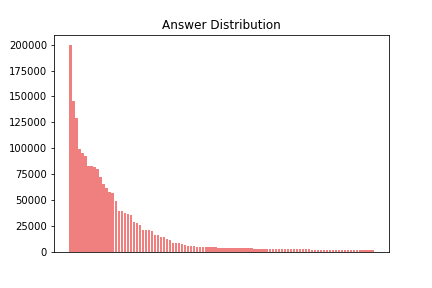
\includegraphics[width=0.8\linewidth]{Figures/answer_dist.png}
\end{center}
   \caption{The distribution of the top 100 answers (excluding "Yes" and "No").}
\label{answer_dist}
\end{figure}


\begin{figure}[t]
\begin{center}
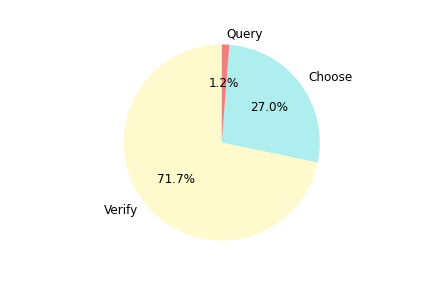
\includegraphics[width=0.8\linewidth]{Figures/struct_dist.png}
\caption{The structural distribution of questions.}
\end{center}
\label{structural}
\end{figure}


\begin{figure}[t]
\begin{center}
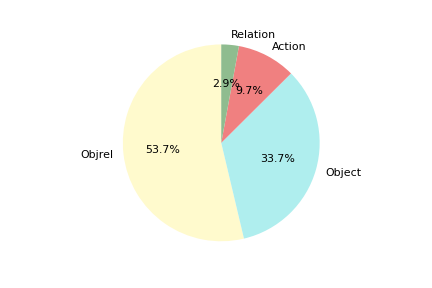
\includegraphics[width=0.8\linewidth]{Figures/sem_dist.png}
\end{center}
   \caption{The semantic distribution of questions.}
\label{semantics}
\end{figure}


\begin{figure}[t]
\begin{center}
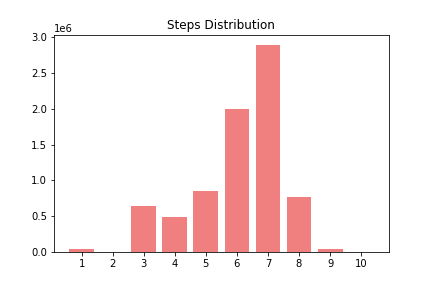
\includegraphics[width=0.8\linewidth]{Figures/steps_dist.png}
\end{center}
   \caption{The distribution of the number of compositional steps.}
\label{steps}
\end{figure}


\begin{figure}[t]
\begin{center}
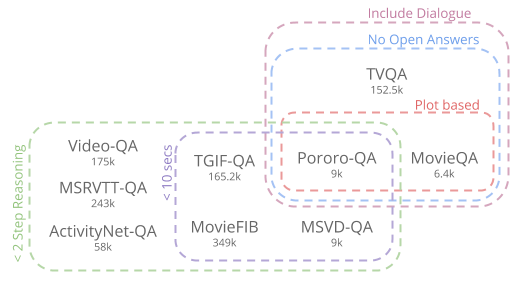
\includegraphics[width=0.8\linewidth]{Figures/figure_videoQA.png}
\end{center}
   \caption{Existing VideoQA benchmarks have some drawbacks. Specifically, many have questions with less than 2 steps of reasoning, using short videos, having plot based questions, only multiple choice questions, and including dialogue.}
\label{existing_benchmarks}
\end{figure}


\begin{figure}[t]
\begin{center}
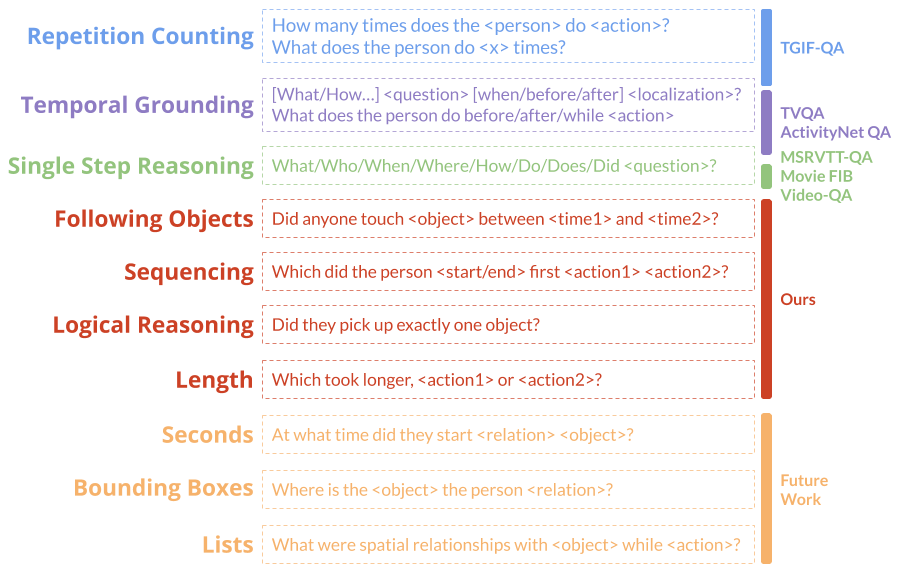
\includegraphics[width=0.8\linewidth]{Figures/figure_temporalTypes.png}
\end{center}
   \caption{Various types of temporal reasoning.}
\label{temporal_types}
\end{figure}


\begin{figure*}[t]
\begin{center}
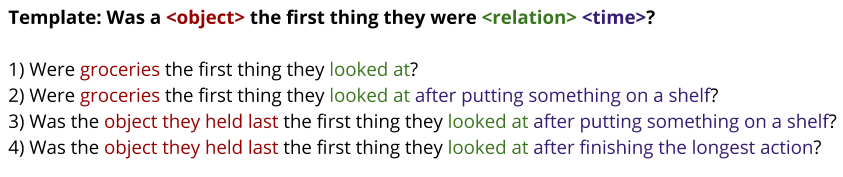
\includegraphics[width=0.8\linewidth]{Figures/figure_indirect.png}
\end{center}
   \caption{Our pipeline uses indirect references to create a variety of questions with different required reasoning steps from the same template. 1) uses all direct references and no temporalization. It has two steps of reasoning (determining if looked at groceries, then finding if that is the first thing at which they looked). 2) Adds temporal localization for a total of 4 steps (localizing when putting something on a shelf, then shifting attention after). 3) Uses an indirect reference for the object, adding one additional step (the last object held) for a total of 5 steps. 4) adds an indirect reference within the temporal localization to add a step (find the longest action) for a question with a total of 6 compositional steps required to answer.}
\label{template_expansion}
\end{figure*}

\begin{figure*}[t]
\begin{center}
%\fbox{\rule{0pt}{2in} \rule{.9\linewidth}{0pt}}
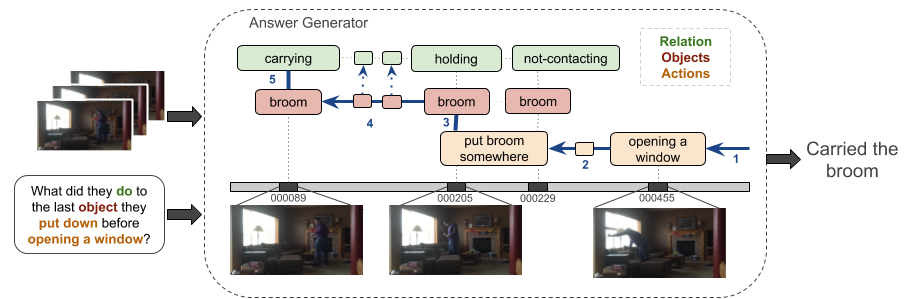
\includegraphics[width=0.8\linewidth]{Figures/figure_questionGenerator.png}
\end{center}
   \caption{The sequence in which our answer generator traverses the spatio-temporal scene graph to automatically generate the answer to a question. The input question can be decomposed into the following spatio-temporal operations: 
  1) localize when the actor opened a window, 
  2) find the last event before then when the actor put an object down, 
  3) determine which object (the broom) was put down, 
  4) look for a different relationship between the actor and this broom, 
  5) Output that the actor ``carried the broom''.}
\label{answer_generator}
\end{figure*}

\begin{figure}[t]
\begin{center}
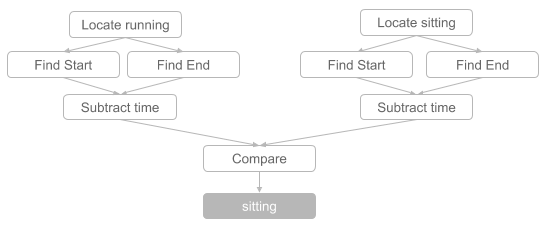
\includegraphics[width=0.8\linewidth]{Figures/figure_composition.png}
\end{center}
   \caption{The substeps required to answer the question "Was the person running or sitting for longer?"}
\label{compositional_substeps}
\end{figure}




%\begin{figure}[t]
%\begin{center}
%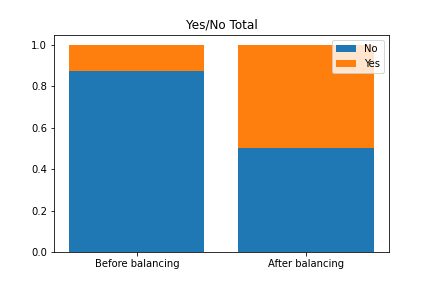
\includegraphics[width=0.8\linewidth]{Figures/yn_total.png}
%\end{center}
%   \caption{The proportion of questions with a Yes/No answer before and after balancing}
%\label{binary_balance}
%\end{figure}


\begin{table}[]
    \begin{center}
    \caption{Suite of Metrics}
    \label{metrics}
    \begin{tabular}{|p{2cm}|p{5cm}|}
     \hline
     \multicolumn{2}{|c|}{\textbf{Content Category}}\\
    \hline
    All & Accuracy on all questions\\
    \hline
    Question Type & Accuracy on each question category (e.g. Counting, Length, First, ...)\\
    \hline
    Answer Type & Accuracy on each answer category (e.g. binary, and open)\\
    \hline
    
    
     \multicolumn{2}{|c|}{\textbf{Generalization}}\\
    \hline
    Video Length & Train on videos of length $<$ 30 seconds. Test on videos of length $\geq$ 30 seconds \\
    \hline
    Actions & Train on videos with $<$ 5 actions. Test on videos with $\geq$ 5 actions  \\
    \hline
    Compositional Steps &  Train on questions with $<$ 6 steps. Test on questions with $\geq$ 6 steps  \\
    \hline
    Novel Compositions & See Table \ref{novel_composition_table} \\
    \hline
    Indirect Consistency & Accuracy on questions referring to the same ideas but using different numbers of indirect references\\
    \hline
    Direct Only & Questions with no indirect refs\\
    \hline
    \% Training Data & Train on only 1, 5, 10 and 20 percent of training data \\
    \hline
    
    
     \multicolumn{2}{|c|}{\textbf{Answer Legitimacy}}\\
    \hline
    Sequencing & Something where sequencing is consistent \\
    \hline
    Consistent & If answers a question correctly, answers all logical entailments correctly \\
    \hline
    Validity & Answer type is of correct genre (e.g. object, relation, action, count, yes/no)\\
    \hline
    Plausibility  & Answer exists in distribution for that question\\
    \hline
    Distribution & Predicted answers follow same distribution as ground truth\\
    \hline
    \end{tabular}
    \end{center}
\end{table}


\begin{table}[]
    \begin{center}
    \caption{Novel Composition}
    \label{novel_composition_table}
    \begin{tabular}{|p{2cm}|p{5cm}|}
    \hline
    \textbf{Name} & \textbf{Novel Combinations} \\
    \hline
    object-relationship & touching table, touching food, beneath table, beneath food\\
    \hline
    repetition & taking a dish from somewhere, putting some food somewhere\\
    \hline
    first/last & looking at first, behind first, holding first \\
    \hline
    before/after & before standing up, before playing with phone, before throwing broom\\
    \hline
    longer & longer than standing up, longer than playing with phone, longer than throwing broom\\
    \hline
    
    \end{tabular}
    
    \end{center}
\end{table}

{\small
\bibliographystyle{ieee_fullname}
\bibliography{dreu_final}
}

\end{document}
\documentclass[10pt,twocolumn,letterpaper]{article}

\usepackage{cvpr}
\usepackage{times}
\usepackage{epsfig}
\usepackage{graphicx}
\usepackage{amsmath}
\usepackage{amssymb}

% Include other packages here, before hyperref.
\newcommand{\rak}[1]{{\color{red}{rak: #1}}}
\newcommand{\ma}[1]{{\color{purple}{ma: #1}}}
\newcommand{\mgm}[1]{{\color{cyan}{mgm: #1}}}

% If you comment hyperref and then uncomment it, you should delete
% egpaper.aux before re-running latex.  (Or just hit 'q' on the first latex
% run, let it finish, and you should be clear).
\usepackage[breaklinks=true,bookmarks=false]{hyperref}

\cvprfinalcopy % *** Uncomment this line for the final submission

\def\cvprPaperID{****} % *** Enter the CVPR Paper ID here
\def\httilde{\mbox{\tt\raisebox{-.5ex}{\symbol{126}}}}

% Pages are numbered in submission mode, and unnumbered in camera-ready
%\ifcvprfinal\pagestyle{empty}\fi
\setcounter{page}{4321}
\begin{document}

%%%%%%%%% TITLE
\title{DREU Final Report: Compositional Spatio-Temporal Reasoning}

\author{Madeleine Grunde-McLaughlin\\
University of Pennsylvania\\
%Philadelphia, Pennsylvania\\
{\tt\small mgrund@sas.upenn.edu}
% For a paper whose authors are all at the same institution,
% omit the following lines up until the closing ``}''.
% Additional authors and addresses can be added with ``\and'',
% just like the second author.
% To save space, use either the email address or home page, not both

\and
Ranjay Krishna\\
Stanford University\\
%Palo Alto, California\\
{\tt\small ranjay.krishna@gmail.com}

\and
Maneesh Agrawala\\
Stanford University\\
%Palo Alto, California\\
{\tt\small maneesh@cs.stanford.edu}


}
\maketitle
\pagestyle{empty}

%%%%%%%%% ABSTRACT
\begin{abstract}
    Existing Video Question Answering benchmarks are limited in the spatio-temporal reasoning skills they measure. We build a pipeline to combine Action Genome's spatio-temporal scene graph annotations with predefined templates to create a new benchmark AGQA. AGQA's question templates create questions that test a wide variety of spatio-temporal reasoning skills, including action sequencing, complex temporal localization, and compositional reasoning \mgm{re-think this list and what is included}. Along with these questions, AGQA contributes an suite of metrics to measure model's accuracy at different reasoning challenges and ability to generalize to more complex tasks. We then test existing models on this new benchmark to measure their relative strengths and weaknesses. \mgm{add results}

\end{abstract}

%%%%%%%%% BODY TEXT


\section{Introduction}

The ability to perceive and reason about the world's actors, actions, objects, and relationships has been a longstanding goal for Computer Vision. Formally, we can benchmark progress towards this goal using tasks like Visual Question Answering, in which a model's reasoning skills are evaluated by it's ability to answer questions about visual stimuli. A variety of benchmarks have been created to test a model's capabilities at answering questions about images~\cite{johnson2017clevr,hudson2019gqa,antol2015vqa,zellers2019recognition,goyal2017making,krishna2017visual,zhu2016visual7w,kim2020answering} and about videos~\cite{tapaswi2016movieqa,lei2018tvqa,jang2017tgif,kim2017deepstory,xu2017video,maharaj2017dataset,zeng2016leveraging,yu2019activitynet}. Ideally, models trained on these benchmarks should be capable of reasoning over both spatial relationships between objects~\cite{krishna2017visual,lu2016visual} and temporal ordering of actions~\cite{zacks2001events,ji2020action}. Unfortunately, since most question-answering benchmarks operate over images, they are limited to only testing spatial relationships (e.g.~``What is on top of the table?'')~\cite{hudson2019gqa,krishna2017visual,antol2015vqa}. The few existing video-only benchmarks have questions with simple temporal logic (e.g.~``What does the bear on right do after sitting?'')~\cite{jang2017tgif,xu2017video,maharaj2017dataset,zeng2016leveraging,yu2019activitynet}. \mgm{Think I need more detail here. Add in cleverer and commonsense reasoning} However, to answer questions that require models to jointly compose spatial and temporal reasoning over multiple steps (e.g.``What did they do to the last object they put down before opening the window?''), we need newer benchmarks and a new class of models.

We introduce the video question answering benchmark Action Genome Question Answering (AGQA) and use it to evaluate models on compositional spatio-temporal reasoning. AGQA measures a wider variety of spatio-temporal reasoning skills than existing benchmarks. An ideal benchmark to measure spatio-temporal reasoning abilities should (1) be free of human annotation bias, (2) use videos of various lengths as input, (3) contain a large number of questions, and (4) provide not just a single accuracy score but a suite of metrics that test various spatio-temporal capabilities. To achieve these goals, we developed an automatic approach that converts Action Genome’s spatio-temporal scene graphs, containing objects, relationships, actors, and actions, into compositional questions~\cite{ji2020action}. \mgm{this list came from the HAI thing, but I'm less convinced now on how important 2-3 are to bring up here. May want to bring up compositionality more explicitly since we've pivoted a bit towards that, but also I'll need to have results probably that show that more compositional questions are harder.}

Existing question-answering benchmarks are limited in the diversity of their questions. Since most benchmarks are image-based, they only test a model's reasoning over spatial relationships~\cite{johnson2017clevr,hudson2019gqa,antol2015vqa,goyal2017making,krishna2017visual,zhu2016visual7w}, object attributes~\cite{johnson2017clevr,hudson2019gqa, antol2015vqa,goyal2017making,krishna2017visual}, and common sense understanding~\cite{zellers2019recognition,antol2015vqa,krishna2017visual}. These benchmarks are unable to test reasoning over temporal relationships or activities. \mgm{clearer common sense specification here}

The questions asked by VideoQA benchmarks that do not include extra textual information like dialogue can be answered from a single frame of the video, apply to the entire video with no temporal localization, or ask "what happened before/after/while $<$action$>$?"~\cite{jang2017tgif,xu2017video, maharaj2017dataset, zeng2016leveraging, yu2019activitynet}. \mgm{a very clunky way of bringing this up. However, I'm not sure how to do it more clearly yet. Think. Also need to address CLEVRER} Temporal localization refers to using the phrase "before/after/while $<$action$>$" to localize a relevant time in the video over which to reason. Beyond the three types of questions listed above, models should be able to perform more complex temporal localization, follow the changing state of objects over time, sequence actions, compare temporal qualities like length among different parts of the video (e.g. "Which activity did they do the longest?"), and generalize to new combinations of ideas~\cite{lake2018generalization,vatashsky2020vqa}. \mgm{re-address this list with the templates we ended up with} Creating this diverse range of questions has previously been difficult. Questions automatically generated from video captions often lack diversity in structure~\cite{yu2019activitynet, jang2017tgif}, while human annotated datasets are too expensive to get a large enough sample to include a wide variety of categories~\cite{zeng2016leveraging, yu2019activitynet}
The community does not know how existing models perform on more complex temporal reasoning and generalization to new content because existing benchmarks do not have questions requiring these abilities. By recursively generating questions with direct references, indirect references, and temporal localizations, our question generation pipeline creates a diverse set of questions that can be trained and tested all together or separated by type. \mgm{making the same pont like 50 different times I want to restructure it a bit to condense all that into one area b/c now it rambles}

An ideal VideoQA benchmark measures the ability to reason over visual stimuli instead of depending on the statistics of answer distributions~\cite{vatashsky2020vqa}. However, many question answering datasets have a bias towards common answers that reduce dependence on visual input and inflate accuracy scores~\cite{goyal2017making, hudson2019gqa}. 
Since we have question content information from our generation pipeline, we are able to smooth the answer distribution among different question types. \mgm{ideally add in numbers about how that makes the blind model worse than blind models on other sets? idk}
An ideal VideoQA benchmark would have videos with a variety of video lengths. Some VideoQA datasets have a variety of clip lengths~\cite{yu2019activitynet,xu2017video}, but most VideoQA datasets use videos of less than 10 seconds long~\cite{jang2017tgif,kim2017deepstory,xu2017video,maharaj2017dataset,zeng2016leveraging,yu2019activitynet}. Some models are better suited for longer or shorter videos, but an ideal model would be able to reason over a variety of lengths~\cite{na2017read,le2020hierarchical}. Although it is expensive to annotate longer clips, we use two already annotated datasets on videos from 2.33 to 194.33 seconds long~\cite{sigurdsson2016hollywood,ji2020action}. \mgm{questionable important this is to talk about lengths of videos}

An ideal VideoQA benchmark should be large. All current VideoQA sets have less than 350K question answer pairs~\cite{jang2017tgif,kim2017deepstory,xu2017video,maharaj2017dataset,zeng2016leveraging,yu2019activitynet,lei2018tvqa,tapaswi2016movieqa}. \mgm{check cleverer} A larger training set can support a wider variety of questions while avoiding underfitting, and a larger testing set can be split into a wider variety of subsets~\cite{maharaj2017dataset}. On only 250 videos, our process generated over 8 million questions of diverse structures. Our final dataset will generate questions on over 9.8K videos. \mgm{no longer as impressively large - probably take out}

Finally, an ideal VideoQA benchmark provides a range of metrics to judge a model's relative strengths and weaknesses. Most existing benchmarks measure accuracy on the overall dataset~\cite{maharaj2017dataset,jang2017tgif,xu2017video,maharaj2017dataset,zeng2016leveraging,yu2019activitynet}. Some also measure accuracy on categories of questions~\cite{jang2017tgif,xu2017video,yu2019activitynet}, or on questions without visual input~\cite{zeng2016leveraging}. For example~\cite{xu2017video} splits questions by the first word ("what", "where", "who", "how, "when"). %, and \cite{jang2017tgif} splits the test set into 1) questions that look at the number of times an action was performed, 2) questions naming the action that occurred X times, 3) questions that use temporal localization, and 4) questions that could be answered from one frame. \mgm{Are these examples helpful or just confusing?}

\mgm{Transition.} Reasoning complexly about videos requires multi-step reasoning, comparative and counting operators, flexibility with video length, appearance feature understanding, and fine and coarse motion understanding~\cite{le2020hierarchical,fan2019heterogeneous}. The accuracy scores of existing benchmarks do not provide the granularity needed to measure success in these different aspects of video understanding~\cite{fan2019heterogeneous,le2020hierarchical}. \mgm{If i going to make this list, I need to back it up more explicitly. I can for all except fine and course motion understanding, so I shoudl take that out} Furthermore, no existing benchmarks we know of measures a model's ability to generalize to new information. AGQA provides a suite of new metrics measuring accuracy by category, the ability to generalize, and the extent to which a model's answers reflect a consistent and realistic understanding of the world. \mgm{Will need to adjust this based on the metrics that I got done. For example, didn't do entailments which was the crux of the "consistent worldview" part. So I probably want to shift the focus to measuring compositional reasoning}

\mgm{Add in final model size and summary of results}

%\mgm{Related work generally: I'm not sure how relevant all the parts are. CLEVR talks about how it balances answers and b/c its synthetic can do more in depth reasoning abilities. GQA talks about balancing answers and how CLEVR is synthetic, and other synthetic question generation methods. So i think focusing more of this section on the previous balancing attempts would help. I'm not sure how important the distinction between ImageQA and VideoQA is. Also neither of them split up the Related work into subsections.}

\section{Related Work}

\subsection{Visual Question Answering}
Visual Question Answering is a task for checking visual reasoning skills by asking a model questions about visual input. 

Image QA is most popular. It works over a variety of inputs (synthetic, real world, charts, cartoons) to measure a variety of concepts (7Ws, common sens reasoning, compositional reasoning, spatial reasoning). It cannot measure temporal reasoning beyond guessing based on common sense.


VideoQA is growing but less explored. First camp looks at text like dialogue and/or focuses on the plot of movies and relationships between characters. This is an interesting question, but often depends on textual input for long term reasoning, so we're looking at vision only. 
CLEVRER is slightly different. It works on synthetic data and focuses on identifying causal relationships. 

Other vision-only, real-world benchmarks ask 3 types of questions 

1) questions that could be answered from a single frame of the video

2) questions that require looking at the whole video (no temporal localization)

3) "What did they do before/after/while <action>?"

They also tend to be small. There is a tradeoff with more complex data that is human generated and therefore expensive, and automatically generated data that has simple logic. 

Ours is vision only and has more complex question structure requiring a wider variety of spatio-temporal reasoning skills. 



\subsection{Automatically Generated Questions}

\mgm{Highly considering taking this section out}

Previous VideoQA datasets have synthetically generated questions from video captions. These questions tend to have simpler temporal logic than human annotated ones. 

GQA and CLEVR both generated questions and were very successful in the ImageQA space. One of the benefits of synthetically generating questions is that you have more control over the content of the questions to make interesting metrics. 

\subsection{Balancing Datasets}
ML models are notoriously good at taking advantage of imbalances in the dataset to improve accuracy scores without using the reasoning skills we want them to. One way of reducing this effect has been balancing the dataset by reducing skews in the answer distribution. 

Has happened in other domains like object detection and image classification, but difficult for question answering from human generated datasets because low control over the content of each question. Also, there are often priors in the existence of certain objects and relationships so that certain question types occur more often than others. 

CLEVR, GQA, and VQA2.0 all attempted balancing. VQA2.0 did it by adding in an similar image with a different answer for 71\% of their dataset. However, after balancing blind models could still answer 67\% of binary question and 27\% of open answer questions without seeing visual input \mgm{our binary is better, but our open is about the same}. 

For VideoQA, ActivityNetQA balanced their yes/no answers and controlled what types of questions were solicited to diversify the distribution of question types. CLEVRER balanced their dataset in a method similar to CLEVR.

Unlike CLEVERER, we are on natural, not synthetic, videos. We also balance more intensely and on a more granular level than existing VideoQA datasets.

\subsection{Compositional Reasoning}

Compositional questions require multiple steps of reasoning to answer (+ example). A constrained set of logical steps can be used as building blocks that are reordered to create a wide variety of queries. 

Humans are able to learn quickly and generalize to new information because they can reason compositionally. 

Compositional questions have been used in ImageQA datasets to rigorously check models because they tend to be longer and more complex. 

Many questions that reason over video require multi-step reasoning (example where reason over time, then about certain thing). We have more complex compositional reasoning than existing real-world datasets.





%\mgm{Overall Methods/Results notes: Clevr talks about be Image and scene representations, image generation, question representations, and question generation. GQA talks more about the question generation pipeline and is closer to what I followed here. Split into four sections 1- scene graph normalization, 2-  question representation 3- functional representation and entailment (we don't have entailment and aren't releasing the programs yet) and 4- sampling and balancing. I think instead of structuring it like i do here where it follows the qualities of the ideal benchmark (which is what we did for HAI) following a more GQA style description of each step in the question generation pipeline may make sense. However, that was also part of their contribution whereas for us, its the tool we used from their contribution. So maybe makes more sense to talk about compositional reasoning and the semantic categories that are time-specific. Also, I'll want to go into the balancing more specifically since i deviated some from the algorithm GQA did.  }


\section{Dataset Generation}

Quick introduction about how this was inspired by GQA, but we expanded it out to the temporal domain and balanced slightly differently. We take the content of spatio-temporal scene graph annotations and use it to fill in natural language question templates.

\subsection{Spatio-temporal Scene graphs}

Quick description of Charades videos. They are 2-194 seconds long, and made by MTurk workers doing skits. Action Genome has spatio-temporal scene graphs, which symbolically represent the objects, subjects, and relationships in Charades videos on a subset of frames. 

These annotations provide the content to fill in the questions. We combine annotations from the two dataset into one combined spatio-temporal scene graph and augment it in several ways. 

\mgm{Im not sure how many of these to include. Will think, and also will depend on space constraints. Some I can move down to supplementary}

1) Dealing with the uncertainty in action segmentation annotation by adding in priors about which actions co-occur and which actions follow each other in sequence

2) Adding in common sense entailments for relationships and objects. For example, if someone is carrying something, they are also holding it and touching it. 

3) Fixing spatial relationships (probably delete this one or put in supplementary)

4) Adding information from co-occurring Charades annotations as objects and relationships in the scene graph. 

5) Combining synonymous words like food and sandwich. (kind of included in number 6)

6) Condensing multiply annotated objects and actions by finding them through IOUs in bounding boxes and time stamps

7) Correlating vague and specific actions in time (e.g. "eating something" and "eating some food") (delete this one)


After making these corrections, our spatio-temporal scene graphs have x objects, y relationships, and z actions. There are 7,787 training set videos and 1814 test set videos that get turned into questions. 


\subsection{Question Templates}

We have a set of x templates. The templates each have a variety of natural language questions with tags indicating what content it needs (example). The spatio-temporal scene graph content is used to fill in those tags. Each template is also associated with a variety of markers about it's content to facilitate balancing and create metrics. Each template is also associated with a program that reasons over the spatio-temporal scene graph to automatically generate the answer. We implement a variety of checks to ensure the questions have high quality. 

\mgm{again, these could go to supplementary}

1) Make sure there is no ambiguity in possible answers

2) Avoid common sense combinations like ("are they wearing clothes?")

3) Avoid questions that give away the answer ("what did they hold while holding a blanket?")

4) Avoiding nonsensical questions (e.g. "Were they eating a mirror?")


\subsection{Creating Compositional Reasoning}

Compositional questions require multiple steps of reasoning to answer. Compositionality comes from the questions themselves, temporal localization, and indirect references. First, certain question structures are more compositional than others (example). Second, many questions localize in time to reference a certain point in the video. These questions require first finding the relevant time in the video, then reasoning over that part. We balanced the dataset to ensure x\% of questions with temporal localization change the answer of the question. Third, sometimes we replace tags with indirect references. In creating the questions, each indirect reference was associated with a program that could be solved first to then reason about the main question.

\subsection{Balancing}

Questions have two answer types, binary and open. Questions are also sorted into global and local categories, similar to GQA (example). For binary questions, we made each local category 50/50 for each answer (example). 

For open questions, we first balanced the global category, then each individual local category. The balancing procedure first truncated 5\% of questions making up the tail of the distribution. \mgm{may want to have a separate algorithm aside to describe this idk. It's a bit of a mouthful} Then, starting with the most popular answer as the "head" it deletes answers in the "head" randomly until either the head / tail proportion, normalized for the number of answers in each, is less than some number b, or if deleting anymore would make an answer x that had been more frequent than answer y less frequent than answer x. Then, the head is expanded to contain an extra answer, and the process repeats. This entire process repeats with b decreasing at every iteration until either half the questions have been deleted, or the first x\% of answers made up less than y\% of all questions. \mgm{Do we need to explain where got the numbers from? It was mostly just experimenting}

    We then balanced on the structural question types. There are five different question structures (explain). Figure for the distribution before and after.

Finally, we balanced so that x\% of questions with a temporal localization change the answer from the question when there is no temporal localization.


\subsection{Results}
Before balancing, was x, y, z. After balancing, was x, y, z (replace with numbers when finish balancing). Figures of how the distributions changed. 



\section{Experiments and analysis}

%CLEVR: First described models. They then analyzed the dataset by question type (query vs compare), relationship type (spatial vs attribute), question topology (chain vs tree-structured questions). they have an interesting section on looking at "effective" question size. They say that accuracy is not necessarily related to question size itself, so they prune functions from the program until they find the smallest functional program that when put on the scene graph creates the correct answer. This is the 'effective' program length, and that is related to difficulty. Nothing comes immediately to mind about how I would do that with AGQA though. They also looked at relative vs absolute spatial reasoning. SO if you say "left of x" they see how accurate it is if you just look in left half of the image, and then they prune when spatial relationships aren't absolutely necessary. They found that much worse on ones that require relative, not absolute, spatial reasoning. This could potentially be expanded to temporal localization. Then look at novel combinations. They have a summary in discussions and future work. 

%GQA: breaks down semantic and structural categories (does not spend much time on these),then talks about data set's vocabulary size and possible answers. We are a lot weaker on this point. GQA talks about briefly baseline experiments on blind models. They they describe transfer performance, i.e. training on VQA and testing on GQA and vice versa to show theirs is harder (we don't have an equivalent though). Then, they get into describing their new metrics and have. subsection for each category. For some of them they have a formal representation, for others they don't.

% Note to self: will need to change some to logical structural.. maybe compare?

%Notes to self: I think that the stuff CLEVR did with pruning down programs to find the essential necessities is cool. I probably don't have time for that now, but worth keeping in mind. 

We created a suite of metrics to measure different types of spatio-temporal and compositional reasoning, then tested them on some models. We found (overall conclusions)


\subsection{Human Analysis}

\mgm{Include this if it's interesting, otherwise, put results in the in the table}

\subsection{Describe the models we looked at briefly}

\mgm{Is it necessary to do this? CLEVR did, GQA did not}

\subsection{Spatio-temporal reasoning capabilities}
\mgm{May need to bring some of these different reasoning types up earlier, but I'm not sure where. Potentially in the templates section, but that is different from methods}

First Paragraph: Global categories. We look at accuracy on different types of reasoning, like count, length, action sequencing, object relationship detection and the superlatives "first" and "last". Put in results we found here. 

Second paragraph: Semantic categories. Put in results about performance on objects vs actions vs relations here. 

\subsection{Question Structure}

We have five types of question structure, query, choose, compare, verify, and logic. Add in results here. 


\subsection{Compositional metrics}

We also create metrics designed to measure compositional reasoning and the ability to generalize. These metrics ask if models, when trained on simpler or incomplete information, can successfully complete a more complex task.

\subsubsection{Novel Composition}

An important part of human reasoning is the ability to generalize concepts of the same category to novel compositions. One way to test this ability in models is to train without a certain combination of phrases, then test to see if it can still correctly reason about that phrase. For example, in the training set the model may never see the phrase "before running", but see both "before" and "running" in other contexts. Then, in the test set, we can test if it understands the  idea  of  ”before running”.   We are able to create such a training and testing split to judge these  novel  compositions  because  we  have  knowledge  of what temporal localization, logical reasoning, and indirect tags are in each question.

Results from models we tested.

\subsubsection{Indirect References}

This metric looks at questions that use only direct references to objects, relationships, and objects with no temporal localization, and sees if the model can still answer identical questions that use indirect references and temporal localizations. Add results here.

\mgm{This will only be interesting if we fix indirects not affecting accuracy.}


\subsubsection{Number of Compositional Steps}

In this section we train the model only on questions with fewer than 6 steps of compositional reasoning, then test on questions with greater than 6 steps. Add results.

\subsubsection{Length of video}

Some video models are better at shorter or longer videos. Many existing video datasets are on short videos and many models are inflexible with video length. This metric tests if models trained on short videos can generalize to being tested on long videos. Add results.


\section{Discussion and Limitations}

\mgm{A lot of separate ideas here, need to find a coherent flow}

Compared to other VideoQA datasets we measure a wider variety of spatio-temporal topics. We also measure compositional reasoning on non-synthetic videos. 

Shortcomings and successes of existing systems (once get results)

Limitation of this generation model to the annotations. Although we did a lot of edits to create high quality questions, some annotation errors will be built into the 

Challenges with having actions as open answers because action segmentation is so uncertain.

Future work could expand to other types of answers, like time stamps, bounding boxes, and lists. Furthermore, future work could expand out from the limited set of objects, relationships, and actions seen in Charades Videos. 

\newpage

\begin{figure}[t]
\begin{center}
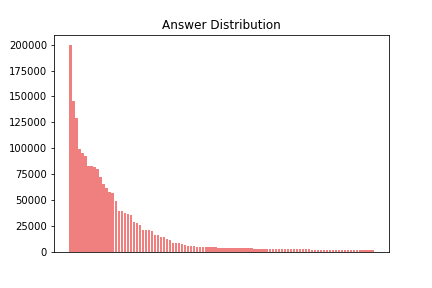
\includegraphics[width=0.8\linewidth]{Figures/answer_dist.png}
\end{center}
   \caption{The distribution of the top 100 answers (excluding "Yes" and "No").}
\label{answer_dist}
\end{figure}


\begin{figure}[t]
\begin{center}
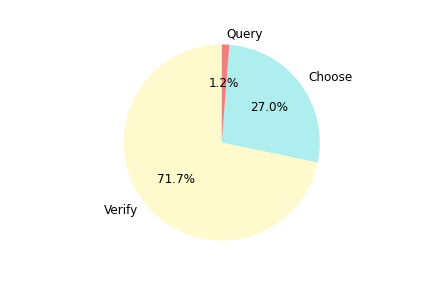
\includegraphics[width=0.8\linewidth]{Figures/struct_dist.png}
\caption{The structural distribution of questions.}
\end{center}
\label{structural}
\end{figure}


\begin{figure}[t]
\begin{center}
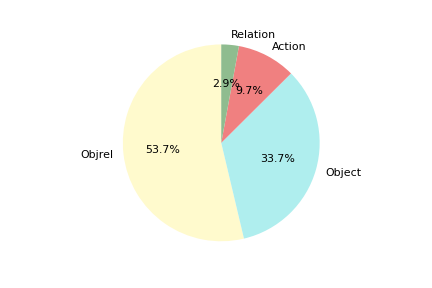
\includegraphics[width=0.8\linewidth]{Figures/sem_dist.png}
\end{center}
   \caption{The semantic distribution of questions.}
\label{semantics}
\end{figure}


\begin{figure}[t]
\begin{center}
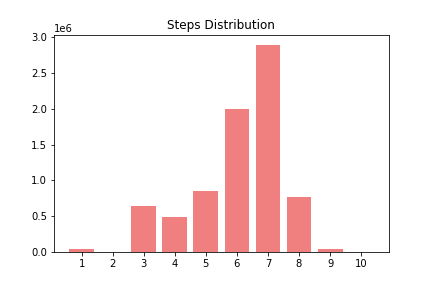
\includegraphics[width=0.8\linewidth]{Figures/steps_dist.png}
\end{center}
   \caption{The distribution of the number of compositional steps.}
\label{steps}
\end{figure}


\begin{figure}[t]
\begin{center}
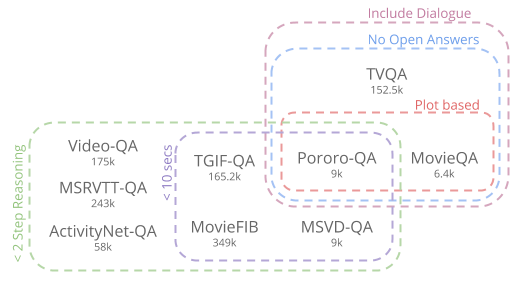
\includegraphics[width=0.8\linewidth]{Figures/figure_videoQA.png}
\end{center}
   \caption{Existing VideoQA benchmarks have some drawbacks. Specifically, many have questions with less than 2 steps of reasoning, using short videos, having plot based questions, only multiple choice questions, and including dialogue.}
\label{existing_benchmarks}
\end{figure}


\begin{figure}[t]
\begin{center}
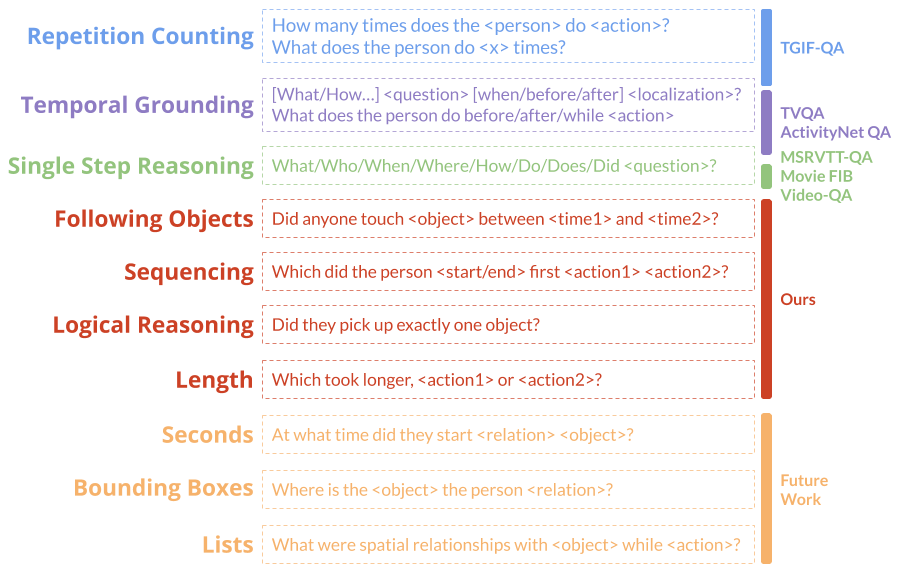
\includegraphics[width=0.8\linewidth]{Figures/figure_temporalTypes.png}
\end{center}
   \caption{Various types of temporal reasoning.}
\label{temporal_types}
\end{figure}


\begin{figure*}[t]
\begin{center}
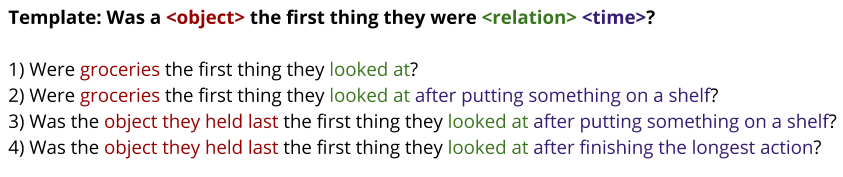
\includegraphics[width=0.8\linewidth]{Figures/figure_indirect.png}
\end{center}
   \caption{Our pipeline uses indirect references to create a variety of questions with different required reasoning steps from the same template. 1) uses all direct references and no temporalization. It has two steps of reasoning (determining if looked at groceries, then finding if that is the first thing at which they looked). 2) Adds temporal localization for a total of 4 steps (localizing when putting something on a shelf, then shifting attention after). 3) Uses an indirect reference for the object, adding one additional step (the last object held) for a total of 5 steps. 4) adds an indirect reference within the temporal localization to add a step (find the longest action) for a question with a total of 6 compositional steps required to answer.}
\label{template_expansion}
\end{figure*}

\begin{figure*}[t]
\begin{center}
%\fbox{\rule{0pt}{2in} \rule{.9\linewidth}{0pt}}
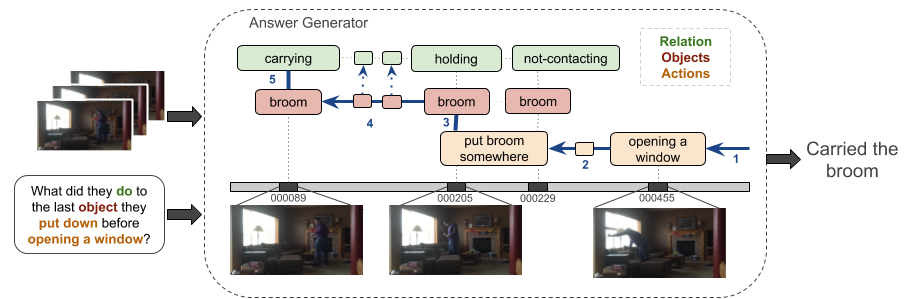
\includegraphics[width=0.8\linewidth]{Figures/figure_questionGenerator.png}
\end{center}
   \caption{The sequence in which our answer generator traverses the spatio-temporal scene graph to automatically generate the answer to a question. The input question can be decomposed into the following spatio-temporal operations: 
  1) localize when the actor opened a window, 
  2) find the last event before then when the actor put an object down, 
  3) determine which object (the broom) was put down, 
  4) look for a different relationship between the actor and this broom, 
  5) Output that the actor ``carried the broom''.}
\label{answer_generator}
\end{figure*}

\begin{figure}[t]
\begin{center}
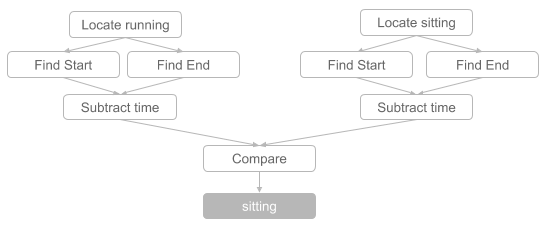
\includegraphics[width=0.8\linewidth]{Figures/figure_composition.png}
\end{center}
   \caption{The substeps required to answer the question "Was the person running or sitting for longer?"}
\label{compositional_substeps}
\end{figure}




%\begin{figure}[t]
%\begin{center}
%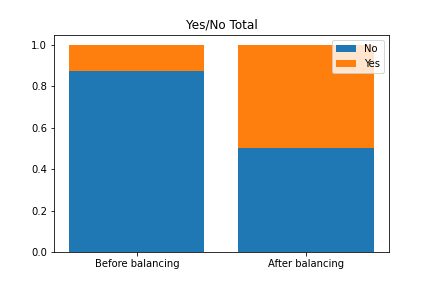
\includegraphics[width=0.8\linewidth]{Figures/yn_total.png}
%\end{center}
%   \caption{The proportion of questions with a Yes/No answer before and after balancing}
%\label{binary_balance}
%\end{figure}


\begin{table}[]
    \begin{center}
    \caption{Suite of Metrics}
    \label{metrics}
    \begin{tabular}{|p{2cm}|p{5cm}|}
     \hline
     \multicolumn{2}{|c|}{\textbf{Content Category}}\\
    \hline
    All & Accuracy on all questions\\
    \hline
    Question Type & Accuracy on each question category (e.g. Counting, Length, First, ...)\\
    \hline
    Answer Type & Accuracy on each answer category (e.g. binary, and open)\\
    \hline
    
    
     \multicolumn{2}{|c|}{\textbf{Generalization}}\\
    \hline
    Video Length & Train on videos of length $<$ 30 seconds. Test on videos of length $\geq$ 30 seconds \\
    \hline
    Actions & Train on videos with $<$ 5 actions. Test on videos with $\geq$ 5 actions  \\
    \hline
    Compositional Steps &  Train on questions with $<$ 6 steps. Test on questions with $\geq$ 6 steps  \\
    \hline
    Novel Compositions & See Table \ref{novel_composition_table} \\
    \hline
    Indirect Consistency & Accuracy on questions referring to the same ideas but using different numbers of indirect references\\
    \hline
    Direct Only & Questions with no indirect refs\\
    \hline
    \% Training Data & Train on only 1, 5, 10 and 20 percent of training data \\
    \hline
    
    
     \multicolumn{2}{|c|}{\textbf{Answer Legitimacy}}\\
    \hline
    Sequencing & Something where sequencing is consistent \\
    \hline
    Consistent & If answers a question correctly, answers all logical entailments correctly \\
    \hline
    Validity & Answer type is of correct genre (e.g. object, relation, action, count, yes/no)\\
    \hline
    Plausibility  & Answer exists in distribution for that question\\
    \hline
    Distribution & Predicted answers follow same distribution as ground truth\\
    \hline
    \end{tabular}
    \end{center}
\end{table}


\begin{table}[]
    \begin{center}
    \caption{Novel Composition}
    \label{novel_composition_table}
    \begin{tabular}{|p{2cm}|p{5cm}|}
    \hline
    \textbf{Name} & \textbf{Novel Combinations} \\
    \hline
    object-relationship & touching table, touching food, beneath table, beneath food\\
    \hline
    repetition & taking a dish from somewhere, putting some food somewhere\\
    \hline
    first/last & looking at first, behind first, holding first \\
    \hline
    before/after & before standing up, before playing with phone, before throwing broom\\
    \hline
    longer & longer than standing up, longer than playing with phone, longer than throwing broom\\
    \hline
    
    \end{tabular}
    
    \end{center}
\end{table}

{\small
\bibliographystyle{ieee_fullname}
\bibliography{dreu_final}
}

\end{document}
